\subsubsection{SICM} 
\paragraph{Overview} The goal of this project is to create a universal interface for discovering, managing and sharing within complex memory hierarchies. The result will be a memory API and a software library which implements it. These will allow operating system, runtime and application developers and vendors to access emerging memory technologies. The impact of the project will be immediate and potentially wide reaching, as developers in all areas are struggling to add support for the new memory technologies, each of which offers their own programming interface. The problem we are addressing is how to program the deluge of existing and emerging complex memory technologies on HPC systems. This includes the MCDRAM (on Intel Knights Landing), NV-DIMM, PCI-E NVM, SATA NVM, 3D stacked memory, PCM, memristor, and 3Dxpoint. Also, near node technologies, such as PCI-switch accessible memory or network attached memories, have been proposed in exascale memory designs. Current practice depends on ad hoc solutions rather than a uniform API that provides the needed specificity and portability. This approach is already insufficient and future memory technologies will only exacerbate the problem by adding additional proprietary APIs. Our solution is to provide a unified two-tier node-level complex memory API. The target users for the low-level interface are system and runtime developers, as well as expert application developers that prefer full control of what memory types the application is using. The high-level interface is designed for application developers who would rather define coarser-level constraints on the types of memories the application needs and leave out the details of the memory management. The low-level interface is primarily an engineering and implementation project. The solution it provides is urgently needed by the HPC community; as developers work independently to support these novel memory technologies, time and effort is wasted on redundant solutions and overlapping implementations. The high-level interface starts with a co-design effort involving application developers. It would potentially evolve into more research as intelligent allocators, migrators, and profiling tools are developed. We can achieve success due to our team’s extensive experience with runtimes and applications. Our willingness to work with and accept feedback from multiple hardware vendors and ECP developers differentiates our project from existing solutions and will ultimately determine the scale of adoption and deployment. 
\begin{figure}
\begin{center}
{
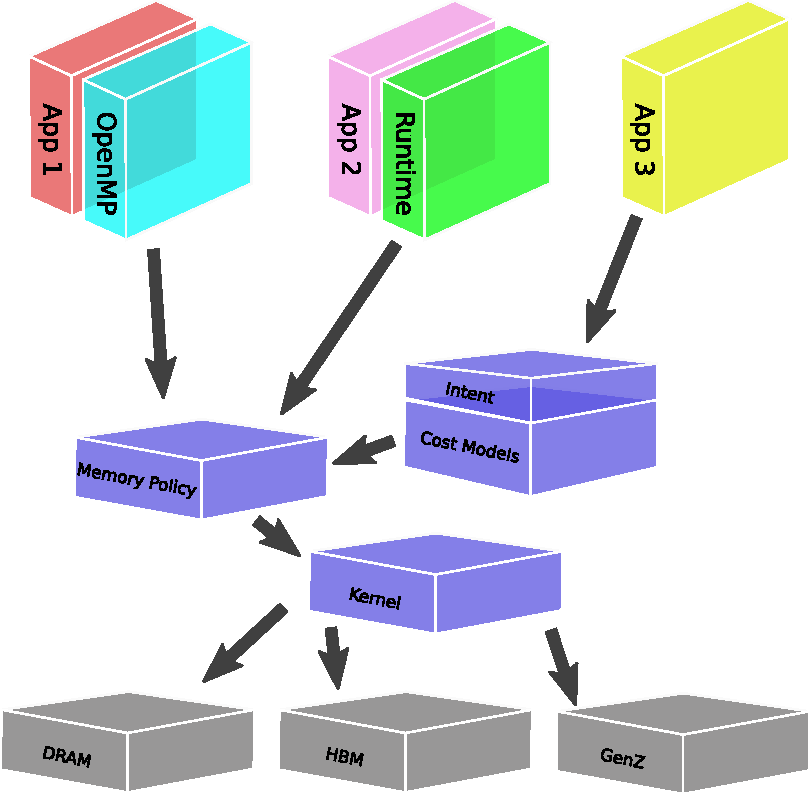
\includegraphics[width=.5\textwidth]{projects/2.3.1-PMR/2.3.1.16-SICM/mike-excelent.pdf}
\caption{Interface for complex memory that is abstract, portable, extensible to future hardware; including a mechanism-based low-level interface that reins in heterogeneity and an intent-based high-level interface that makes reasonable decisions for applications}
}
\end{center}
\end{figure}

\paragraph{Key  Challenges}
This effort is a new start and relies on interaction and acceptance of both the vendors and various runtime libraries. Defining a common mechanism to expose various heterogeneous memory devices is important but vendors have not little adopted a standard in this area and will have to be led to a solution. 

\paragraph{Solution Strategy}

The deliverable of this project is the userspace libraries and modifications to the Linux kernel~\cite{Williams:2017:NDH:3145617.3145620} to that would allow better use of heterogeneous memories. The low-level interface would provide support for discovery, allocation/de-allocation, partitioning, and configuration of the memory hierarchy and information on the properties of each specific device (capacity, latency, bandwidth, volatility, power usage, etc.). The interface will be quickly prototyped for a small set of currently available memory technologies (both volatile and non-volatile) and delivered to runtime and application developers, as well as vendors, for feedback on its functionality, performance and features. The high-level interface will leverage the low-level library in order to further decouple applications from hardware configurations. Specifically, it would emphasize ease of use by application developers with a policy/intent driven syntax enabled through run-time intelligence and system support. Applications would specify which attributes (such as fast, low latency, high capacity, persistent, or reclaimable) are a priority for each allocation and the interface will provide the most appropriate configuration. Finally, the missing element is a common set of functions that would constitute a minimal hardware interface to the various types of memory. The goal is to allow fast porting to new hardware but still leave room for innovation by vendors.



\paragraph{Recent Progress}
\begin{itemize}
\item Low-Level Interface: Progressing on the refactoring of the initial SICM userspace library. Developed the data structure and implementation to track the memory pages in different arenas.
High-Level Interface: 
\item High-Level Interface: Completed initial API design for new high-level SICM persistent memory meta allocator, now called "Metall".   Design heavily leverages open-source Boost.Interprocess, and retains some compatibility with it.  
\item Analysis: Ongoing meetings with Ompi-X team members at Univ. of Tennessee to discuss memory needs and SICM requirements.
\item Analysis: evaluating new static analysis capabilities in the Portland Group compiler that generates comprehensive relationship data of both data structures and functions. The results for ACME are stored in a database. As of this quarter, we can now reliably tie trace references back to a line of code via the database.
\item Analysis: evaluating ACME using Gem5. We are currently resolving some compatibility issues between the ACME build environment and our Gem5 virtual machine. We now have traces from ES3M and several mini-apps.
\item Analysis: Efforts to analyze E3SM and mini-apps using tools by Cray and Intel. These results will be combined with previous results to help characterize barriers and gaps based on feedback from the E3SM team.
\item Cost Models: We have extracted a lot of experimental data related to application memory use and layout. This was done with full applications on hardware with the memory throttling-based emulation methodology. Additionally we have finer grained measurements for smaller C benchmarks where we have isolated individual data structures and applied different tiering decisions to assess metrics such as sensitivity, benefit, etc. More of a tool and profiling process to inform the design of the a simple API/API extension that you might integrate with the running application.~\cite{Doudali:2017:CTE:3132402.3132418}

\item Cost Models: Development of a tool, Mnemo, which provides for automated recommendations of capacity sizing of heterogeneous memories for object store workloads. Given a platform with specific configuration of different memories, and a (representative) workload, we can quickly extract some of the relevant memory usage metrics, and produce cost-benefit estimation curves as a function of different capacity allocations of the different types of memories. The output of Mnemo are estimates which give its users information to make informed decisions about capacity allocations. This can have practical use in shared/capacity platforms, or to rightsize capacity allocations to collocated workloads. 
\end{itemize}
\paragraph{Next Steps}
\begin{itemize}
	\item  Low-Level Interface: Finish implementation of refactor and test with proxy applications for functionality and correctness. Investigate Linux kernel modifications for page migration in collaboration with ECP project Argo 2.3.5.05 and RIKEN research center in Japan. Verify support of emerging OpenMP standards.
\item High-Level Interface: Continuing to work on completing first working prototype; performance testing to follow after prototype is complete.   Initial performance benchmarks have been selected, including a key-value store with skewed key frequency distribution.   These benchmarks also serve as part of a correctness validation test set.
\item Document needs of MPI and ACME climate app hybrid memory analysis (with ORNL collaborators and related to UNITY)
\item Understand capabilities of hwloc and netloc with respect to OMPI-X needs.
Future planned reports will include assessments of what the new SICM tools provide compared to current tools using ACME as a benchmark. The missing gaps are used by the SICM team to inform R/D directions.	
\end{itemize}


